\section{Multivariate analysis}

The event selection described in~\Cref{sec:event_selection} only
serves as a pre-selection to select events following the the expected
topology of the signal processes, and ensuring that basic requirements
on kinematic properties of final state objects are fulfilled. %
% , ensuring trigger efficiencies are in saturation,
The signal-to-background ratio at this level of selection, with
background being three orders of magnitude more abundant than the
expected non-resonant \HH signal in the \hadhad channel
(cf.~\Cref{tab:hadhad_presel_yields}), is not sufficient to provide
any signal sensitivity.

The non-resonant and resonant production of Higgs boson pairs have
distinct kinematic properties that can be used to reject backgrounds
in the signal region. An example, largely independent of the \HH
production mode, are the reconstructed invariant masses of Higgs boson
decay products. A number of reconstructed quantities can be defined
that offer discrimination power to distinguish between the various
signals and backgrounds.

Multivariate methods are used to exploit the discrimination power of
multiple reconstructed quantities and their correlations, classifying
events regarding their similarity to the signal and background
processes. Depending on the \HH production mode and analysis category
different methods are used.

The search for non-resonant \HH production in the SM uses Boosted
Decision Trees and Neural Networks to distinguish between signal and
background in the \hadhad and \lephad channel, respectively. When
searching for resonant \HH production in BSM scenarios, multiple mass
hypotheses for the scalar resonance decaying into Higgs boson pairs
are considered. The kinematics of final state particles in signal
events are dependent on the mass of the resonance, \mX, and as a
result the classification task continuously varies with \mX. This is
in contrast to the former case where the kinematic properties of
signal events follow from a fixed distribution. Classification tasks
that vary as a function of a physical or theoretical parameter, for
example the mass of a resonance, can be performed by \emph{Parametric
  Neural Networks} (PNN) and were first introduced to HEP
in~\cite{Baldi:2016fzo}. PNN provide a single classifier that is able
to handle multiple classification tasks described by one or multiple
parameters, while being able to smoothly interpolate to parameter
values not seen during training of the network.

The scores provided by these multivariate classification methods,
hereafter called MVA scores, are later used as a discriminant in
maximum likelihood fits to extract the signal of interest, setting
upper limits on signal strengths and cross-sections. No further
selections are applied to events entering the signal extraction
procedure such that the pre-selection regions are also signal regions
of the respective channels.

\Cref{sec:mva_crossvalidation} begins by describing the cross
validation method used to ensure that model selection and MVA
predictions are unbiased.  In~\Cref{sec:mva_discriminating variables}
the choice of discriminating variables to classify signal and
background processes will be motivated. Afterwards, the training and
optimisation of the classifiers used to extract non-resonant signal is
described in~\Cref{sec:mva_smbdt}. Finally, \Cref{sec:mva_pnn}
describes the classification using PNN and their main properties.


\subsection{Cross validation method}
\label{sec:mva_crossvalidation}

Many machine learning algorithms, due to their ability to approximate
large classes of functions, are susceptible to fitting statistical
fluctuations in the data that are used to train a model. As a result,
predictions of performance characteristics of the model based on the
training data might not generalise to previously unseen data. In
extreme cases, frequently called overfitting, the performance of the
model evaluated on an independent dataset starts to degrade when
further increasing the capacity of the model~\cite{hastie09}.

When using multivariate methods in searches for new physics, it has to
be ensured that the methods are evaluated on a dataset that was not
used for training or model selection (the process of choosing the
model to fit), thus providing an estimate of the generalised
performance. In this analysis, events are categorised according to
their event number into even- and odd-numbered events, yielding an
even- and odd-fold, respectively. The training and model selection can
proceed by using one of the two folds withholding the remaining fold
for later evaluation. This procedure is applied twice by using each
fold for training once.

After model selection and training, the models are evaluated by
applying the model trained on the even-fold on odd-numbered events and
the model trained on the odd-fold on even-numbered events. This
approach, which is called 2-fold \emph{cross
  validation}~\cite{hastie09,bishop06}, provides an unbiased
evaluation of the MVA scores using the entirety of the available
dataset. The same evaluation method is applied to signal region data
recorded by the ATLAS detector, which is not part of the training
procedure.

Similar to the biased predictions obtained when evaluating
multivariate methods on datasets used for training, the process of
model selection needs to be performed on a dataset that is independent
of the one used for final evaluation of the
method~\cite{cawley10}. Model selection is the process of choosing a
particular configuration of an algorithm (or between different
algorithms), for example input variables and other hyperparameters,
based on a metric indicating the performance of the model. Making this
choice based on the performance on the withheld dataset meant for
later evaluation will introduce a selection bias and represents a form
of overfitting.

In this search the model selection is performed using 5-fold cross
validation (CV), which is a generalisation of the 2-fold approach
described previously to a larger number of subdivisions, separately on
even- and odd-numbered events. This approach effectively nests
5-fold CV inside of 2-fold CV and is therefore called
\emph{nested cross validation}~\cite{cawley10,stone74}.

\Cref{fig:cross_validation} shows a schematic description of one
iteration of the nested cross validation approach. The inner,
5-fold CV randomly splits events into five disjoint subsets
(folds). For every choice of fold used to evaluate the model, the
model is trained on the remaining four folds, subsequently evaluating
the trained model on the evaluation-fold. A decision between two
competing models can be made by comparing the average and standard
deviation of a metric over the five iterations of the inner CV. Only
after the best-performing model is selected, usually after re-fitting
the model on all five folds, it is evaluated on the hold-out dataset.

\begin{figure}[htbp]
  \centering

  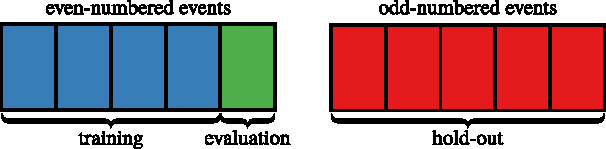
\includegraphics[scale=1]{mva/kfold}

  \caption{5-fold cross validation approach for model selection on
    even-numbered events. The separation of events into disjoint
    subsets (folds) is indicated by rectangles. The purpose of the
    subset is denoted below. A single step out of a total of five, the
    number of possible assignments of the evaluation fold, is
    shown. The hold-out dataset is not used for model selection.}
  \label{fig:cross_validation}
\end{figure}


\subsection{Discriminating variables}
\label{sec:mva_discriminating variables}

The set of variables provided to multivariate classification methods
is crucial to its performance in distinguishing between classes. The
initial choice of variables considered in this search is based on a
previous publication in the same analysis channel by the ATLAS
collaboration using a partial dataset of \SI{36.1}{\ifb} recorded
during Run~2 of the LHC~\cite{HIGG-2016-16-witherratum}. Only minor
changes to the variable choice are performed for this search.

The kinematic features of Higgs boson pair production allow to
distinguish it from the main backgrounds in the \bbtautau search
channel. Candidates for the products of
$\PHiggs \ra \Pbottom\APbottom$ and $\PHiggs \ra \tautau$ decays are
reconstructed (cf.~\Cref{sec:reconstruction_of_higgs_candidates}) and
can be used to estimate four-momenta of Higgs bosons in signal
events. Among the most important variables distinguishing between
signal and background processes are \PHiggs- and \HH-system invariant
masses.

The Missing Mass Calculator (MMC)~\cite{Elagin:2010aw} is used to
reconstruct the four-momentum of the Higgs boson candidate decaying
into pairs of \tauleptons, thus providing an estimate of the
$\tau\tau$-system mass, \mMMC. The mass resolution of the MMC ranges
from \SIrange{15}{18}{\GeV} for signal processes depending on the
momentum of the Higgs boson in the \hadhad channel\footnote{The
  presence of an additional neutrino in the \lephad channel makes mass
  reconstruction of the $\tau\tau$-system more difficult degrading the
  mass resolution of the MMC.}.

The invariant mass of the $\PHiggs \ra \Pbottom\APbottom$ candidate,
consisting of two \btagged jets, is reconstructed using the
four-momenta of both jets after $b$-jet momentum correction
(cf.~\Cref{sec:bjet_momentum_corrections}). For the considered signal
processes the Higgs boson mass can be reconstructed with a resolution
of \SIrange{13}{18}{\GeV}.

The performance of the \PHiggs mass reconstruction is summarised
in~\Cref{fig:mass_reconstruction_H} for the resonant production \HH as
a function of the resonance mass. The broad peaks in the \mMMC and
\mBB spectra close to the Higgs boson mass allow to select signals
with high efficiency while providing large rejection power against
most SM backgrounds. Both \PHiggs-system masses are used as inputs to
the MVAs in all analysis categories.\todo{Move to event selection
  reconstruction / section?}

\begin{figure}[htbp]
  \centering

  \begin{subfigure}[t]{.5\textwidth}
    \centering
    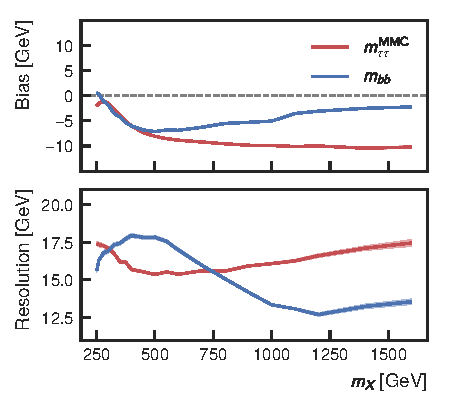
\includegraphics{mva/mass_resolution}
    \caption{\PHiggs-system mass reconstruction}
    \label{fig:mass_reconstruction_H}
  \end{subfigure}\hfill%
  \begin{subfigure}[t]{.5\textwidth}
    \centering
    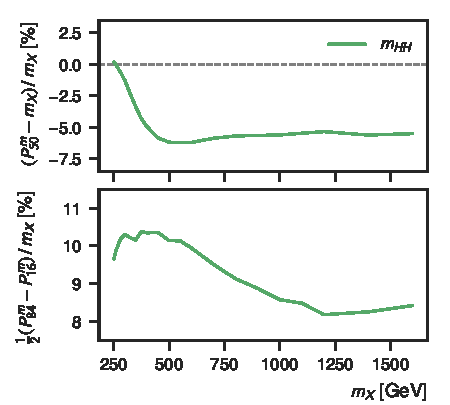
\includegraphics{mva/mhh_resolution}
    \caption{\HH-system mass reconstruction}
    \label{fig:mass_reconstruction_HH}
  \end{subfigure}

  \caption{Performance of methods used to reconstruct the
    \PHiggs-system mass (a) and the \HH-system mass (b) in the \hadhad
    SR estimated using simulation of $\PX \ra \HH \ra \bbtautau$
    processes. The top panels show the median mass prediction,
    $P_{50}^{m}$, of the respective method. The bottom panels show
    half the difference between the 84th and 16th percentile as an
    estimate of the resolution. For the \HH-system reconstruction,
    these quantities are shown relative to the mass of the resonance.}
  \todo[inline]{Add error. Should say sth.\ about the bias and
    behaviour.}
  \label{fig:mass_reconstruction}
\end{figure}

The invariant mass of the decay products of both Higgs bosons, \mHH,
provides another discriminant used in all analysis categories. It is
determined from the sum of four-momenta of the
$\Ptauon\APtauon$-system, reconstructed using the MMC, and
$\bbbar$-system, calculated as the sum of $b$-jet candidate
four-momenta after $b$-jet momentum correction. With a typical mass
resolution of \SIrange{8}{10}{\percent} relative to the mass of the
resonance and the prevalence of most backgrounds at low values of
\mHH, it provides an important discriminant in the search for \HH in
the resonant production mode.

Higgs bosons originating from signal processes are typically produced
with large momenta in the \HH rest frame, the exception being \HH
production via resonances with masses close to the \HH production
threshold, leading to a small angular separation of the (visible)
\PHiggs decay products. The distances \dRtautau and \dRbb between the
visible decay products of the \taulepton and $b$-jet candidate pair,
respecively, provide discrimination power against multi-jet and top
pair production where \taulepton and $b$-jet candidates are less
collimated.
% , except for \dRbb in \lephad LTT,

In a given analysis category the multivariate methods use the same
input variables to extract \HH signal in the resonant and non-resonant
production modes. The choice of variables differs between categories
and is summarised in~\Cref{tab:mva_inputvar}. A brief description of
variables used in the \lephad channel is given in the following.
Reconstructed electrons and muons are collectively referred to as
leptons ($\ell$).
\begin{description}

\item[$\Delta \pT(\ell, \tauhadvis)$] The transverse momentum
  difference between lepton and \tauhadvis.

\item[\mTW] Transverse mass of the \PW boson for processes where
  \pTmiss solely originates from the decay $\PW \ra \ell \nu_\ell$ defined as:
  $\mTW = \sqrt{2 |\pT^{\ell}| |\pTmiss| \cos(1 - \Delta\phi)}$.

\item[\pTmiss $\phi$ centrality] A measure of the relative angular
  position of \pTmiss and visible \taulepton decay products
  (electrons, muons, or \tauhadvis) in the transverse plane. The
  measurement is relative to the line bisecting the azimuthal angle
  between the pair of visible \taulepton decay products and can be
  defined as~\cite{HIGG-2013-32, HIGG-2016-16-witherratum}:
  \begin{align*}
    \pTmiss\text{ }\phi\text{ centrality} = \frac{A + B}{\sqrt{A^2 + B^2}} \text{,}
  \end{align*}
  where
  \begin{align*}
    A = \frac{\sin(\phi_{\pTmiss} - \phi_{\tau_1})}{\sin(\phi_{\tau_2} - \phi_{\tau_1})} \qquad B = \frac{\sin(\phi_{\tau_2} - \phi_{\pTmiss})}{\sin(\phi_{\tau_2} - \phi_{\tau_1})} \text{,}
  \end{align*}
  with $\phi_{\pTmiss}$ and $\phi_{\tau_1}$ / $\phi_{\tau_2}$ denoting
  the azimuthal angle of \pTmiss and visible \taulepton decay
  products, respectively.

  The \pTmiss $\phi$ centrality reaches a maximum of $\sqrt{2}$
  (minimum of $-\sqrt{2}$) when \pTmiss is aligned with the bisecting
  line, pointing into the smaller (larger) angle spanned by the pair
  of visible \taulepton decay products. In configurations where
  \pTmiss is collinear with one of the visible \taulepton decay
  products it takes a value of 1.

\item[$\Delta\phi(\ell\tauhadvis, bb)$] Azimuthal angle between the
  $\ell + \tauhadvis$ system and the system consisting of the two
  \bjet candidates.

\item[$\Delta\phi(\ell, \pTmiss)$] Azimuthal angle between the lepton
  and \pTmiss.

\item[$\Delta\phi(\pTauTau, \pTmiss)$] Azimuthal angle between
  $\tau\tau$-system, reconstructed using the MMC, and \pTmiss.

\item[$s_{\text{T}}$] The effective mass of the event defined as the
  scalar sum of tranverse momenta of all selected jets, \tauhadvis,
  leptons, and \pTmissAbs.
\end{description}

\begin{table}[htbp]
  \centering

  \begin{tabular}{
  l
  >{\centering\arraybackslash}p{2cm}
  >{\centering\arraybackslash}p{2cm}
  >{\centering\arraybackslash}p{2cm}
  }
  \toprule
  & \multicolumn{3}{c}{Analysis Channel} \\ \cmidrule{2-4}
  Variable                              & \hadhad    & \lephad SLT & \lephad LTT \\
  \midrule
  \mMMC                                 & \checkmark & \checkmark & \checkmark \\[0.1em]
  \mBB                                  & \checkmark & \checkmark & \checkmark \\[0.1em]
  \mHH                                  & \checkmark & \checkmark & \checkmark \\[0.1em]
  \dRtautau                             & \checkmark & \checkmark & \checkmark \\[0.1em]
  \dRbb                                 & \checkmark & \checkmark &            \\[0.1em]
  $\Delta \pT(\ell, \tauhadvis)$        &            & \checkmark & \checkmark \\[0.1em]
  Sub-leading $b$-jet \pT               &            & \checkmark &            \\[0.1em]
  \mTW                                  &            & \checkmark &            \\[0.1em]
  \pTmissAbs                            &            & \checkmark &            \\[0.1em]
  \pTmiss $\phi$ centrality             &            & \checkmark &            \\[0.1em]
  $\Delta\phi(\ell\tauhadvis, bb)$      &            & \checkmark &            \\[0.1em]
  $\Delta\phi(\ell, \pTmiss)$           &            &            & \checkmark \\[0.1em]
  $\Delta\phi(\pTauTau, \pTmiss)$       &            &            & \checkmark \\[0.1em]
  $s_{\text{T}}$                         &            &            & \checkmark \\
  \bottomrule
 \end{tabular}


%%% Local Variables:
%%% mode: latex
%%% TeX-master: "../phd_thesis.tex"
%%% End:


  \caption{Discriminating variables used by the multivariate
    classifiers distinguishing between events originating from signal
    and background processes in all three analysis categories. The
    same input variables are used for the search in the non-resonant
    and resonant production modes.}
  \label{tab:mva_inputvar}
\end{table}

The \pTmiss $\phi$ centrality, previously used in the \hadhad
channel~\cite{HIGG-2016-16-witherratum}, was not found to contribute
to the classification performance when comparing models with cross
validation in the \hadhad channel. It is therefore removed as an input
to the multivariate analysis of the \hadhad channel.

All five discriminating variables used in the \hadhad channel are
shown in~\Cref{fig:mva_inputs}. A selection of variables used in the
\lephad SLT and LTT channels are documented
in~\cite{ATLAS-CONF-2021-030}.


% \Cref{fig:mva_input_correlations}

\begin{figure}[htbp]
  \centering

  \begin{subfigure}[t]{.48\textwidth}
    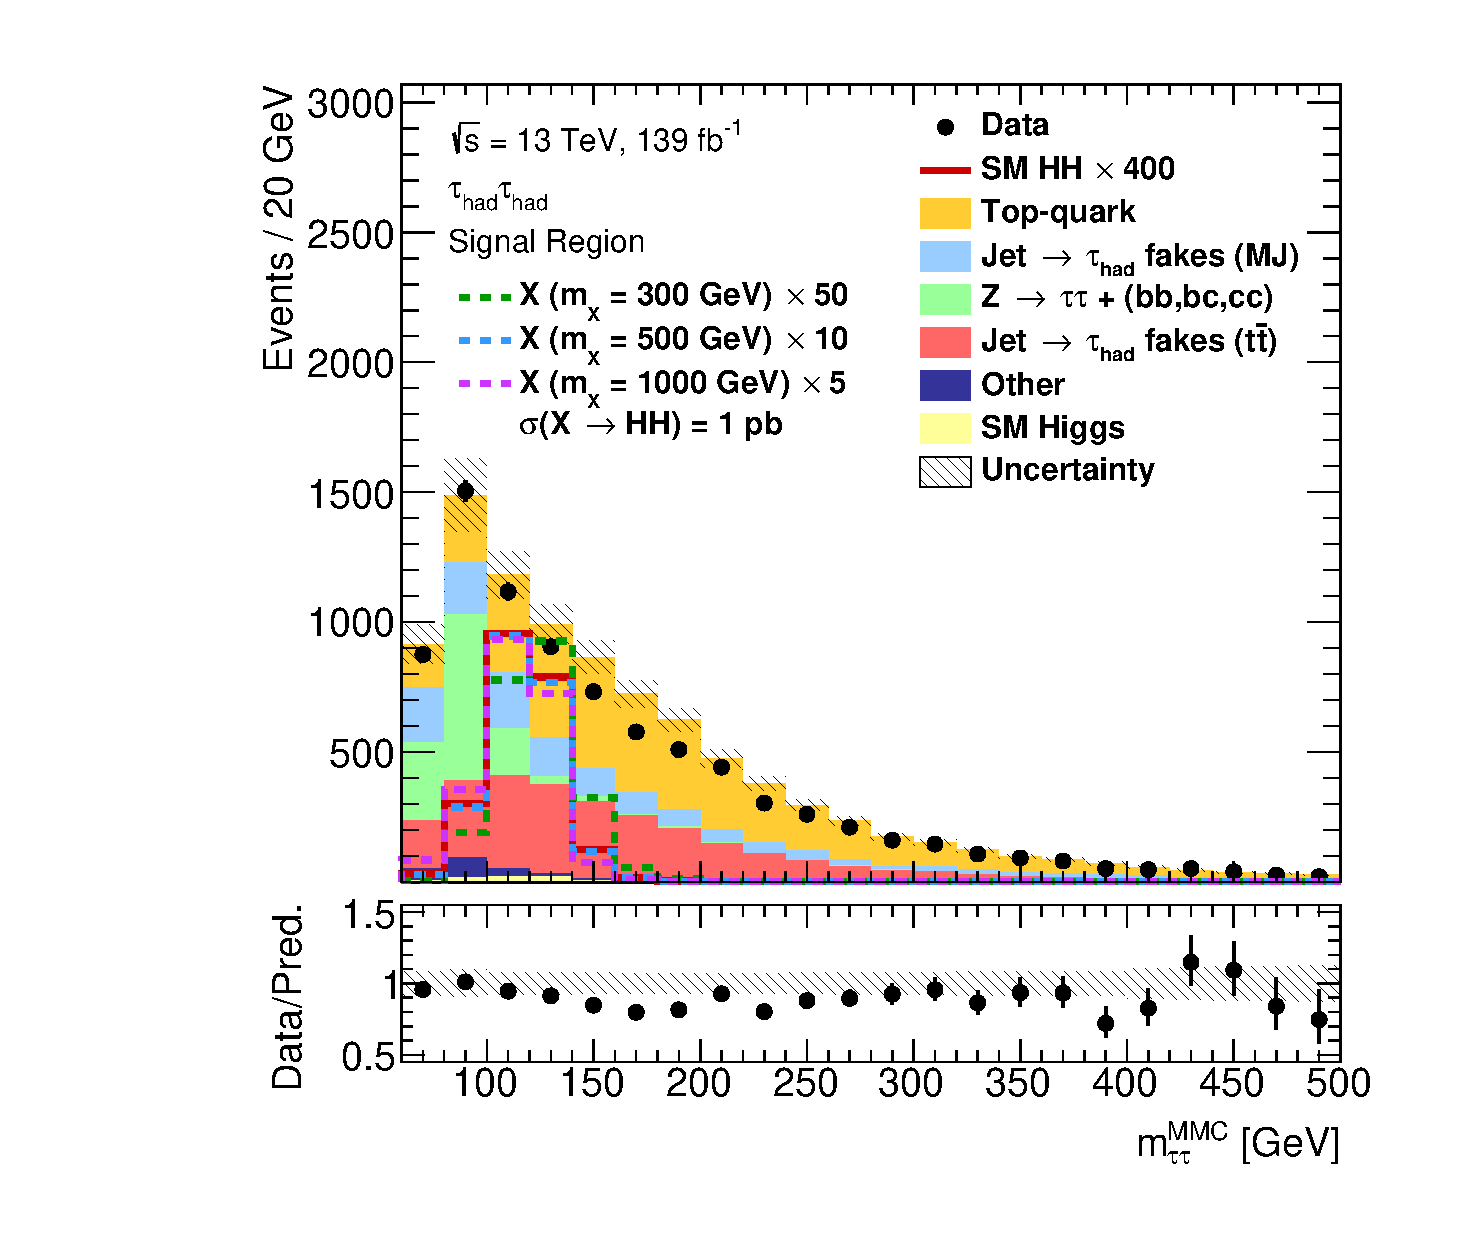
\includegraphics[width=\textwidth]{mva/prefit/Region_BMin0_incJet1_distmMMC_J2_Y2015_DLLOS_T2_SpcTauHH_L0_Prefit}
  \end{subfigure}\hfill %
  \begin{subfigure}[t]{.48\textwidth}
    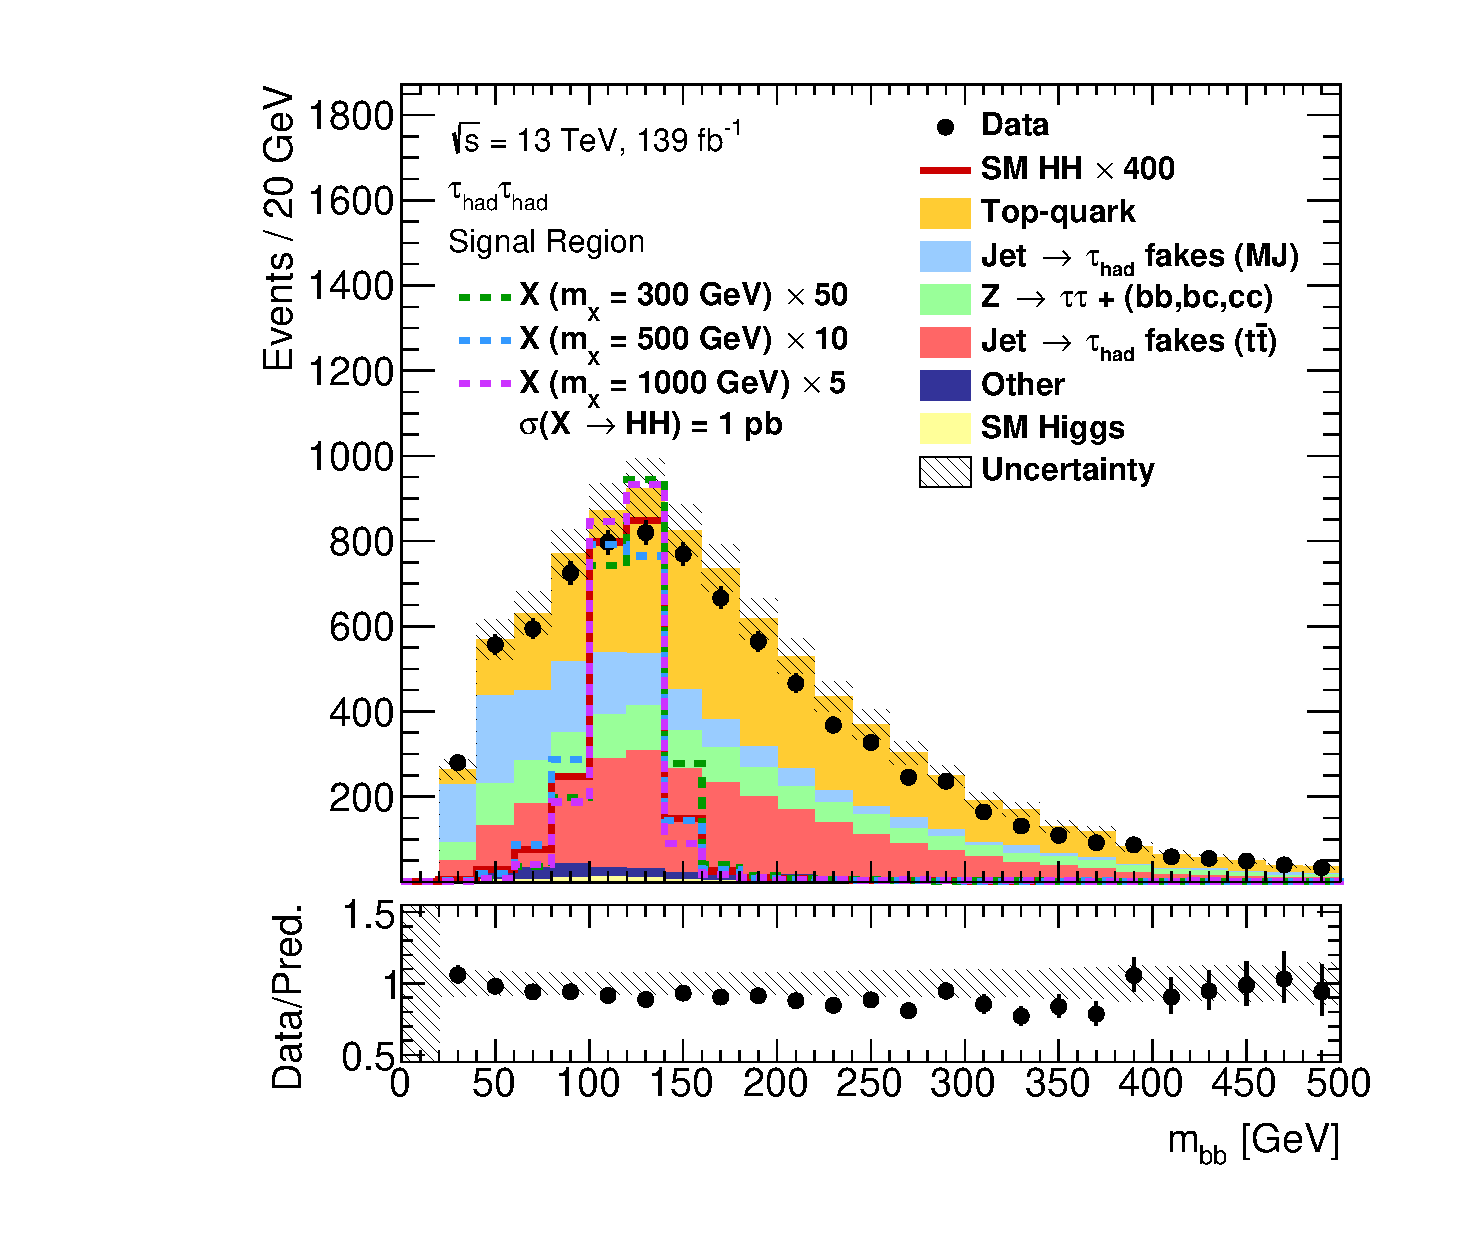
\includegraphics[width=\textwidth]{mva/prefit/Region_BMin0_incJet1_distmBB_J2_Y2015_DLLOS_T2_SpcTauHH_L0_Prefit}
  \end{subfigure}

  \begin{subfigure}[t]{.48\textwidth}
    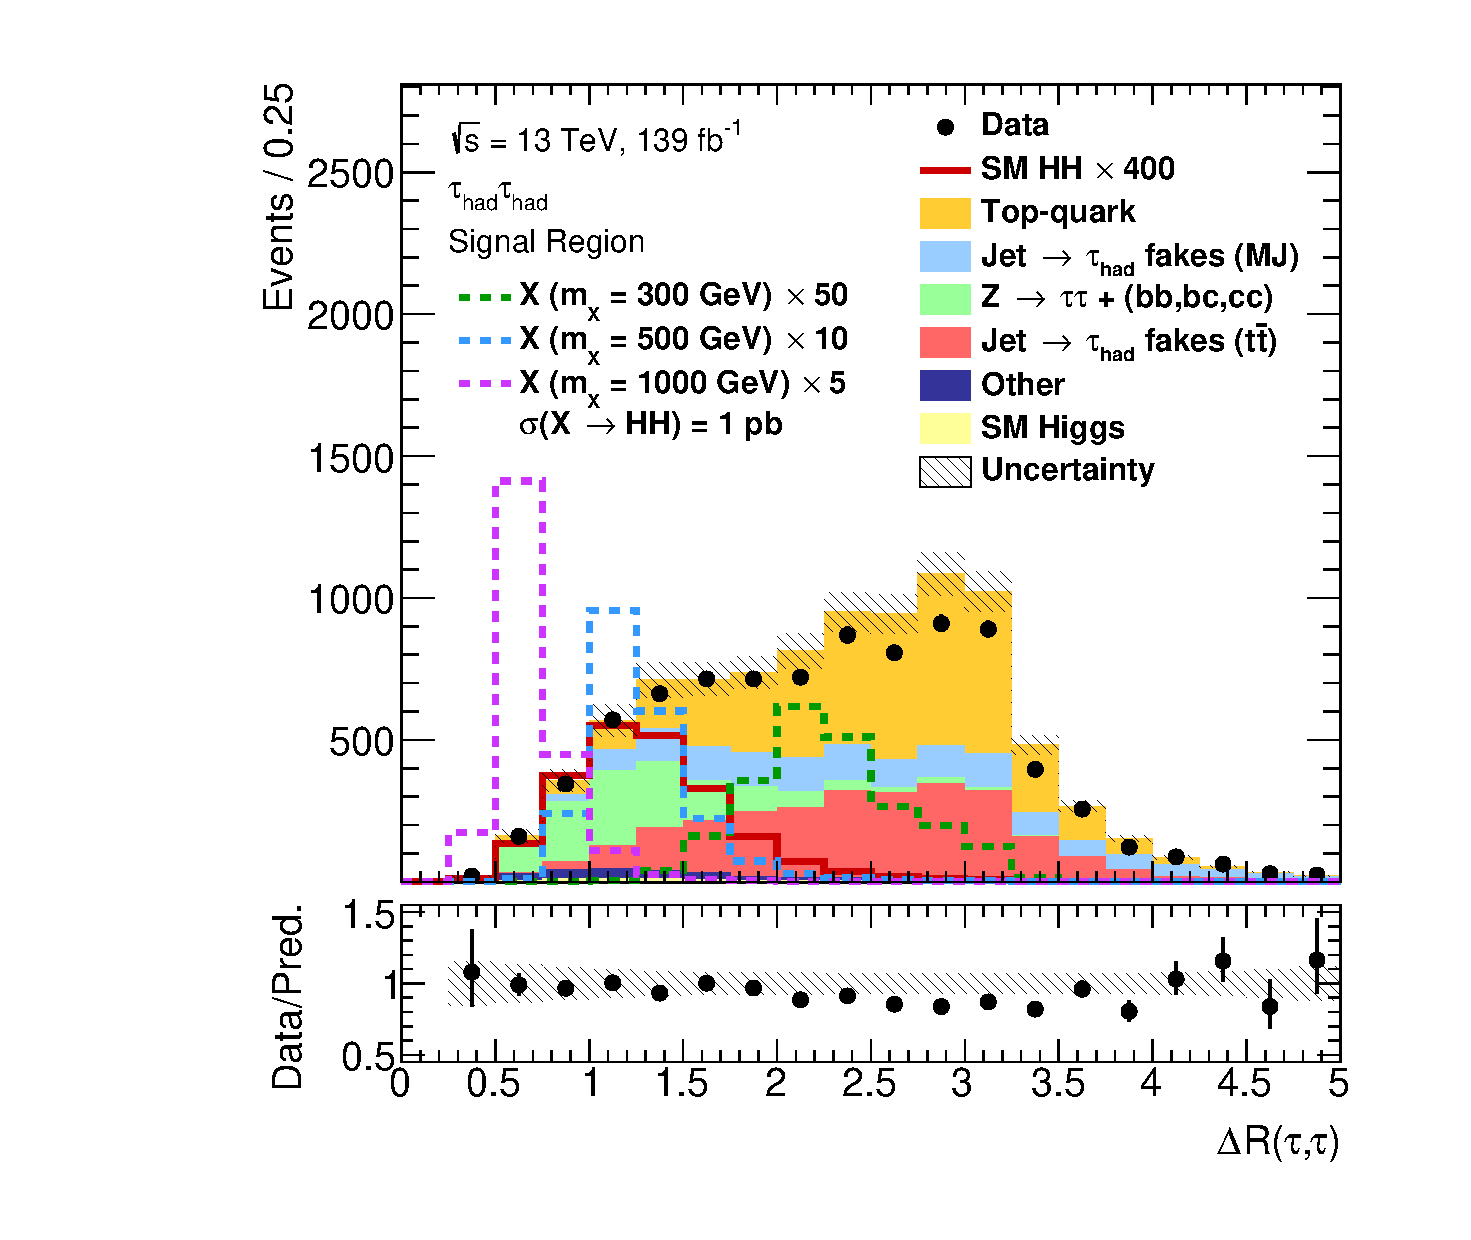
\includegraphics[width=\textwidth]{mva/prefit/Region_BMin0_incJet1_distdRTauTau_J2_Y2015_DLLOS_T2_SpcTauHH_L0_Prefit}
  \end{subfigure}\hfill %
  \begin{subfigure}[t]{.48\textwidth}
    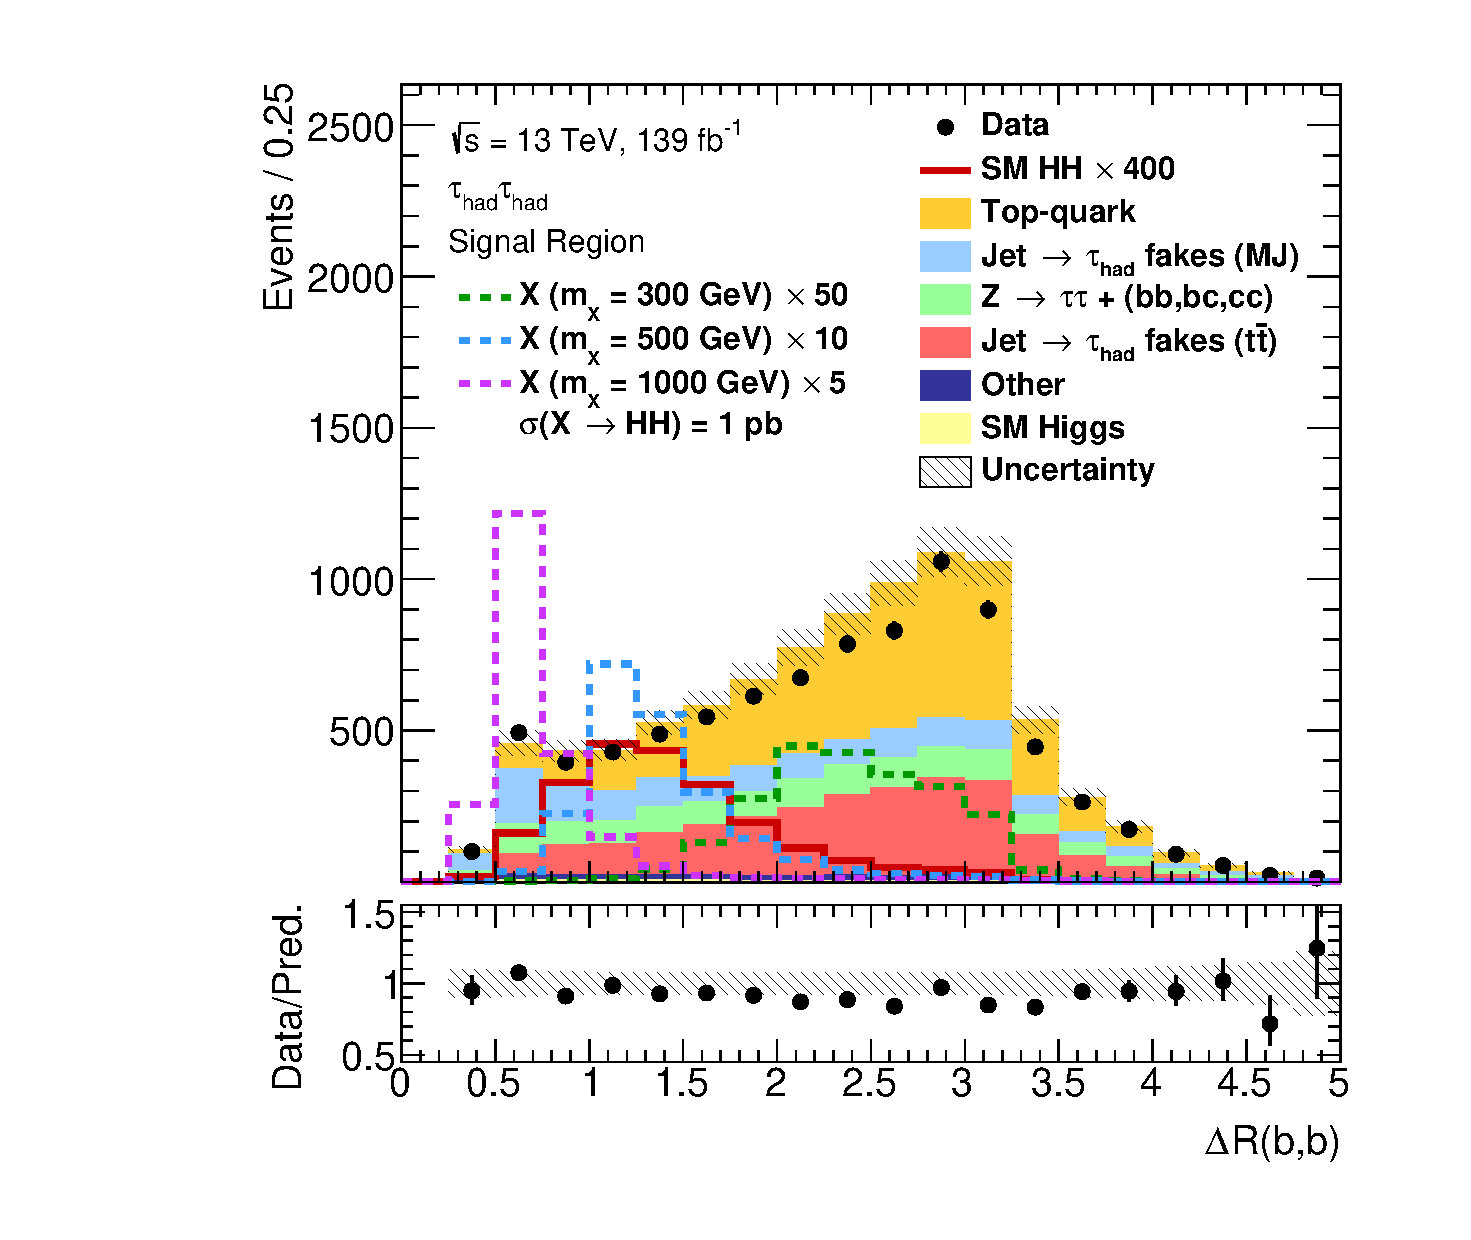
\includegraphics[width=\textwidth]{mva/prefit/Region_BMin0_incJet1_distdRBB_J2_Y2015_DLLOS_T2_SpcTauHH_L0_Prefit}
  \end{subfigure}

  \begin{subfigure}[t]{.48\textwidth}
    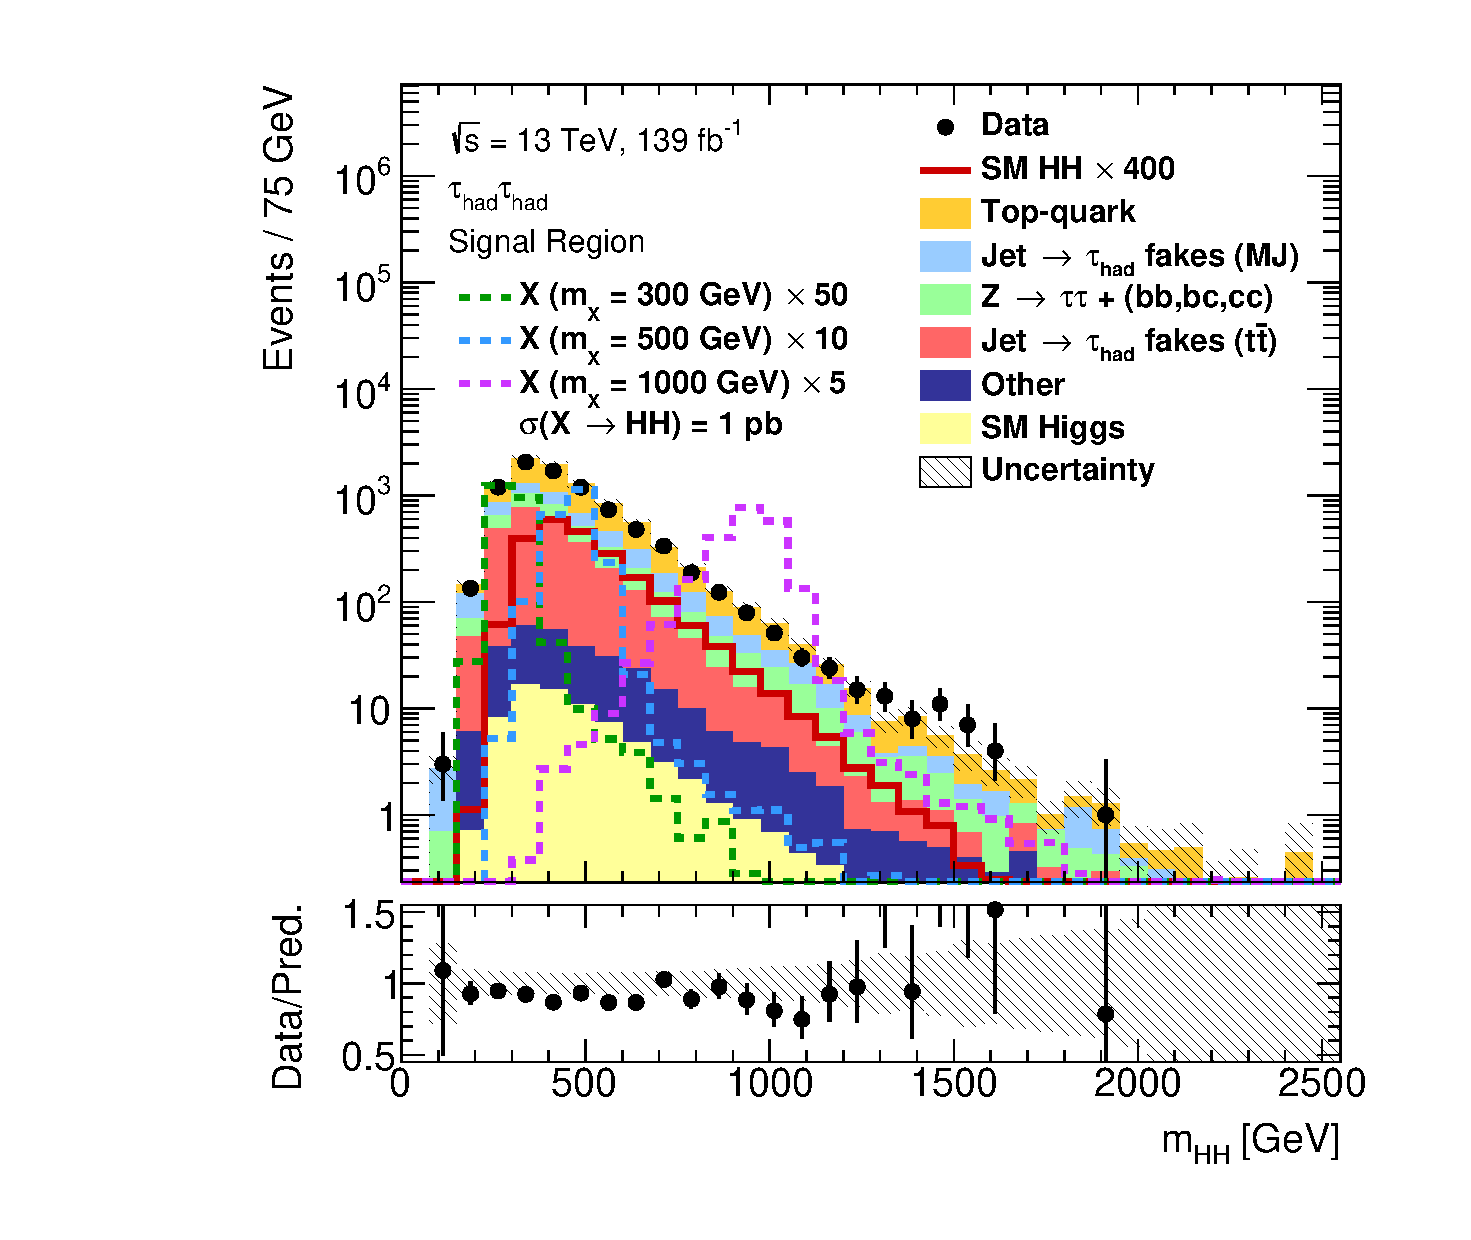
\includegraphics[width=\textwidth]{mva/prefit/Region_BMin0_incJet1_distmHH_J2_Y2015_DLLOS_T2_SpcTauHH_L0_Prefit_logy}
  \end{subfigure}

  \caption{Distributions of the MVA input variables in the SR of the
    \hadhad channel prior to the maximum likelhood fit. The
    uncertainty bands include all statistical and systematic
    uncertainties of the background model. The resonant and
    non-resonant \HH signals are scaled by arbitrary factors for
    visibility.}
  \label{fig:mva_inputs}
\end{figure}


\begin{figure}[htbp]
  \centering

  \begin{subfigure}[t]{.49\textwidth}
    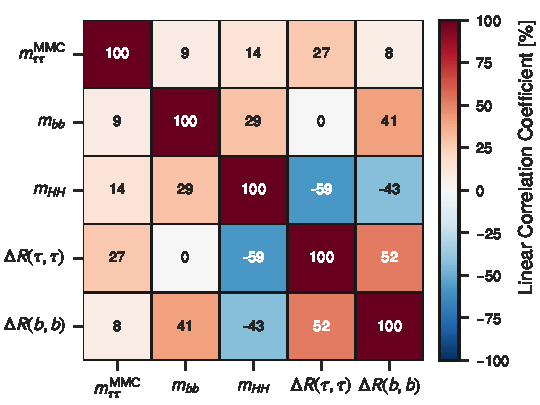
\includegraphics[width=\textwidth]{mva/correlations/NonResHH_pearson}
    \caption{SM \HH (gluon fusion)}
  \end{subfigure}\hfill %
  \begin{subfigure}[t]{.49\textwidth}
    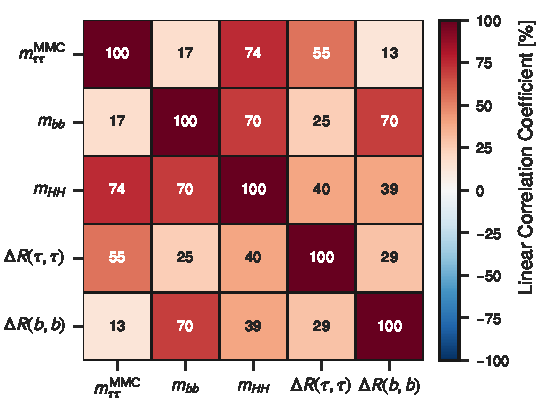
\includegraphics[width=\textwidth]{mva/correlations/ttbar_pearson}
    \caption{\ttbar}
  \end{subfigure}

  \begin{subfigure}[t]{.49\textwidth}
    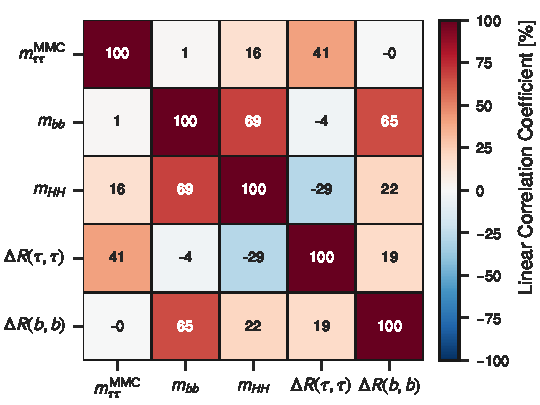
\includegraphics[width=\textwidth]{mva/correlations/Ztautau_pearson}
    \caption{$Z \rightarrow \tautau + \text{jets}$}
  \end{subfigure}\hfill %
  \begin{subfigure}[t]{.49\textwidth}
    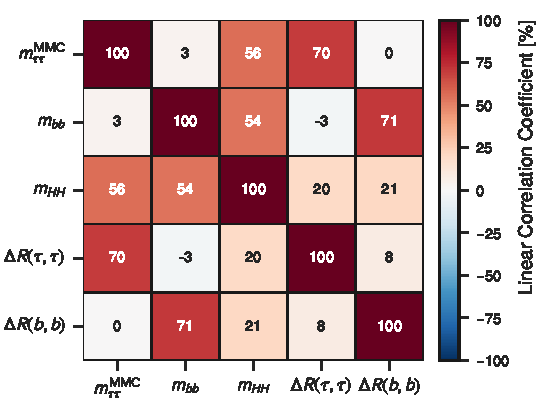
\includegraphics[width=\textwidth]{mva/correlations/Fake_pearson}
    \caption{Multi-jet}
  \end{subfigure}

  \caption{Correlation matrices of the MVA input variables for the SM
    \HH signal and the three largest background contributions (b) -
    (d) in the \hadhad SR.}
  \label{fig:mva_input_correlations}
  \todo[inline]{Cite in text and interpret (or move
    appendix). Different 'correlation patterns' between these
    backgrounds can be used in multivariate methods to better classify
    signal from background.}
\end{figure}


\subsection{Extraction of the non-resonant \HH production using
  Boosted Decision Trees in the \hadhad channel}
\label{sec:mva_smbdt}

The extraction of the non-resonant \HH signal is performed by training
BDT to perform binary classification distinguishing the SM \HH signal
from background. Events in the 2~$b$-tag pre-selection region of the
\hadhad channel are used to train the BDT. The training uses
simulation of the non-resonant \HH production via gluon fusion as the
\emph{signal class}; the combination of all backgrounds considered in
the analysis as the \emph{background class}.  The individual
background processes, which are estimated from simulation or data
(multi-jet), are weighted according to their relative
cross-sections. The SM \HH production via vector boson fusion is not
included due to the its low cross-section compared to the gluon fusion
production mode. The implementation of the BDT algorithm in the
\emph{Toolkit for Multivariate Data Analysis}
(TMVA)~\cite{Hocker:2007ht} is used.


\subsubsection{Hyperparameter optimisation}

The configuration of the BDT is optimised using a random search on a
grid of parameter values. For every hyperparameter of the algorithm a
set of parameter values to test is defined. All possible combinations
define a grid from which configurations are drawn randomly. The
expected performance of the configuration is evaluated using 5-fold
cross validation separately on even- and odd-numbered events.

The hyperparameter values considered for the optimisation are listed
in~\Cref{tab:hyperparameter_grid_bdt}. The total weight of signal and
background events in the BDT training are ensured to be equal by
rescaling of the event weights prior to training. The decision tree
algorithm uses the Gini index as the splitting criterion, testing 400
different thresholds on input variables for every branching of the
tree. Other settings remain at the default values of
TMVA~v4.2.1~(ROOT~6.16/00).

\begin{table}[htbp]
  \centering
  \begin{tabular}{ll}
  \toprule
  Hyperparameter & Values considered \\
  \midrule
  Number of trees & 200, 400, 800, 1000, \underline{1500}, 2000 \\[0.1em]
  Tree depth & 1, \underline{2}, 3 \\[0.1em]
  Minimum node size & \SI{0.01}{\percent}, \SI{0.1}{\percent}, \underline{\SI{1}{\percent}}, \SI{5}{\percent} \\[0.1em]
  Boosting algorithm & \underline{Gradient Boosting}, AdaBoost \\[0.1em]
  Learning rate & 0.01, 0.02, 0.04, 0.08, 0.1, 0.15, \underline{0.2}, 0.3, 0.4 \\[0.1em]
  Ignore negatively weighted events & \underline{Yes}, No \\
  \bottomrule
\end{tabular}

%%% Local Variables:
%%% mode: latex
%%% TeX-master: "../phd_thesis"
%%% End:

  \caption{Hyperparameter values considered for the random grid search optimising the performance of the BDT used to select the non-resonant \HH signal. The underlined values show the final configuration after optimisation.}
  \label{tab:hyperparameter_grid_bdt}
\end{table}

The metric used for optimisation is the area under the \emph{receiver
  operating characteristic} curve (ROC-AUC). The ROC curve can be
defined
% \footnote{The ROC curve relates the true positive rate
%   ($\varepsilon_\text{s}$) and false positive rate
%   ($\varepsilon_\text{b}$) given varying thresholds on the output of a
%   binary classifier. The definition used here uses conventions
%   commonly used in HEP to express this relationship.}
as the parametric curve given by
$(x, y) = \left( \varepsilon_{\text{s}}(t), 1 -
  \varepsilon_{\text{b}}(t) \right)$, where $t$ is a lower threshold
applied on the score of a classifier, and $\varepsilon_\text{s}$ /
$\varepsilon_\text{b}$ the signal and background efficiency of this
selection, respectively. A value of the ROC-AUC of $1$ indicates
perfect classification, while a value of $1/2$ corresponds to an
uninformative classifier. The ROC-AUC is chosen as the metric to be
optimised as it summarises the classifier's performance over all
possible working points, i.e.~choices of thresholds on the classifier
output~\cite{james13}.

In total, approximately 1600 unique BDT configurations are tested
during the model selection process. The steps described in the
following are applied on the datasets containing even- and
odd-numbered events separately. The 5-fold CV approach described
in~\Cref{sec:mva_crossvalidation} is used to evaluate the performance
of a given hyperparameter configuration. For a fixed configuration the
ROC-AUC average and standard deviation is calculated over all
iterations of the CV.

Out of all evaluated configurations, the ROC-AUC of the 200 best
performing model configurations are statistically indistinguishable
based on the CV results. In the absence of a clearly preferred
configuration, the highest ranking configuration with the smallest
maximum tree depth is chosen. A smaller tree depth, effectively
limiting the number variable interactions used in the
classifier~\cite{hastie09}, is chosen to be less reliant on the
quality of the modelling of higher order variable interactions in the
training data.

The selected configuration, shown underlined
in~\Cref{tab:hyperparameter_grid_bdt}, is the 5th and 7th highest
ranking one with a ROC-AUC of \num{0.9803 +- 0.0008} and \num{0.9787
  +- 0.0012} in CV on even- and odd-numbered events, respectively. In
both cases the same configuration ranks highest among models with a
maximum tree depth of 2.  After choosing the configuration, the
classifiers are re-trained on all five folds of the inner CV,
providing the final classifiers to extract the SM \HH signal.

It should be noted that the model selection should be done
independently on both outer folds of the CV, typically leading to two
different configuration choices for even- and odd-numbered events, to
be free of model selection bias. The decision rule was not fixed a
priori, thus it cannot be excluded that the results informed the final
decision. This effect, however, is assumed to be negligible given the
large overlap of the best ranking configurations.

% The BDT classifier was also compared to an optimised feedforward
% neural network, following the approach taken in the \lephad
% channel. The optimised NN could not outperform the BDT, although it
% provided comparable classification performance, thus it was decided to
% use the BDT for the final analysis.


\subsubsection{Predictive performance and variable importance}

In~\Cref{fig:mva_smbdt_prefit} the combined distribution of both BDT,
which are evaluated on events withheld from training and model
selection, is shown in the 2 $b$-tag pre-selection region of the
\hadhad channel. The BDT score provides good separation power between
the SM \HH signal and most background processes. The ROC-AUC of the
final evaluation is \num{0.9772 +- 0.0004} (\num{0.9781 +- 0.0004})
when including (excluding) the SM \HH production via vector boson
fusion, similar to the estimates from cross validation during model
selection.

\begin{figure}[htbp]
  \centering

  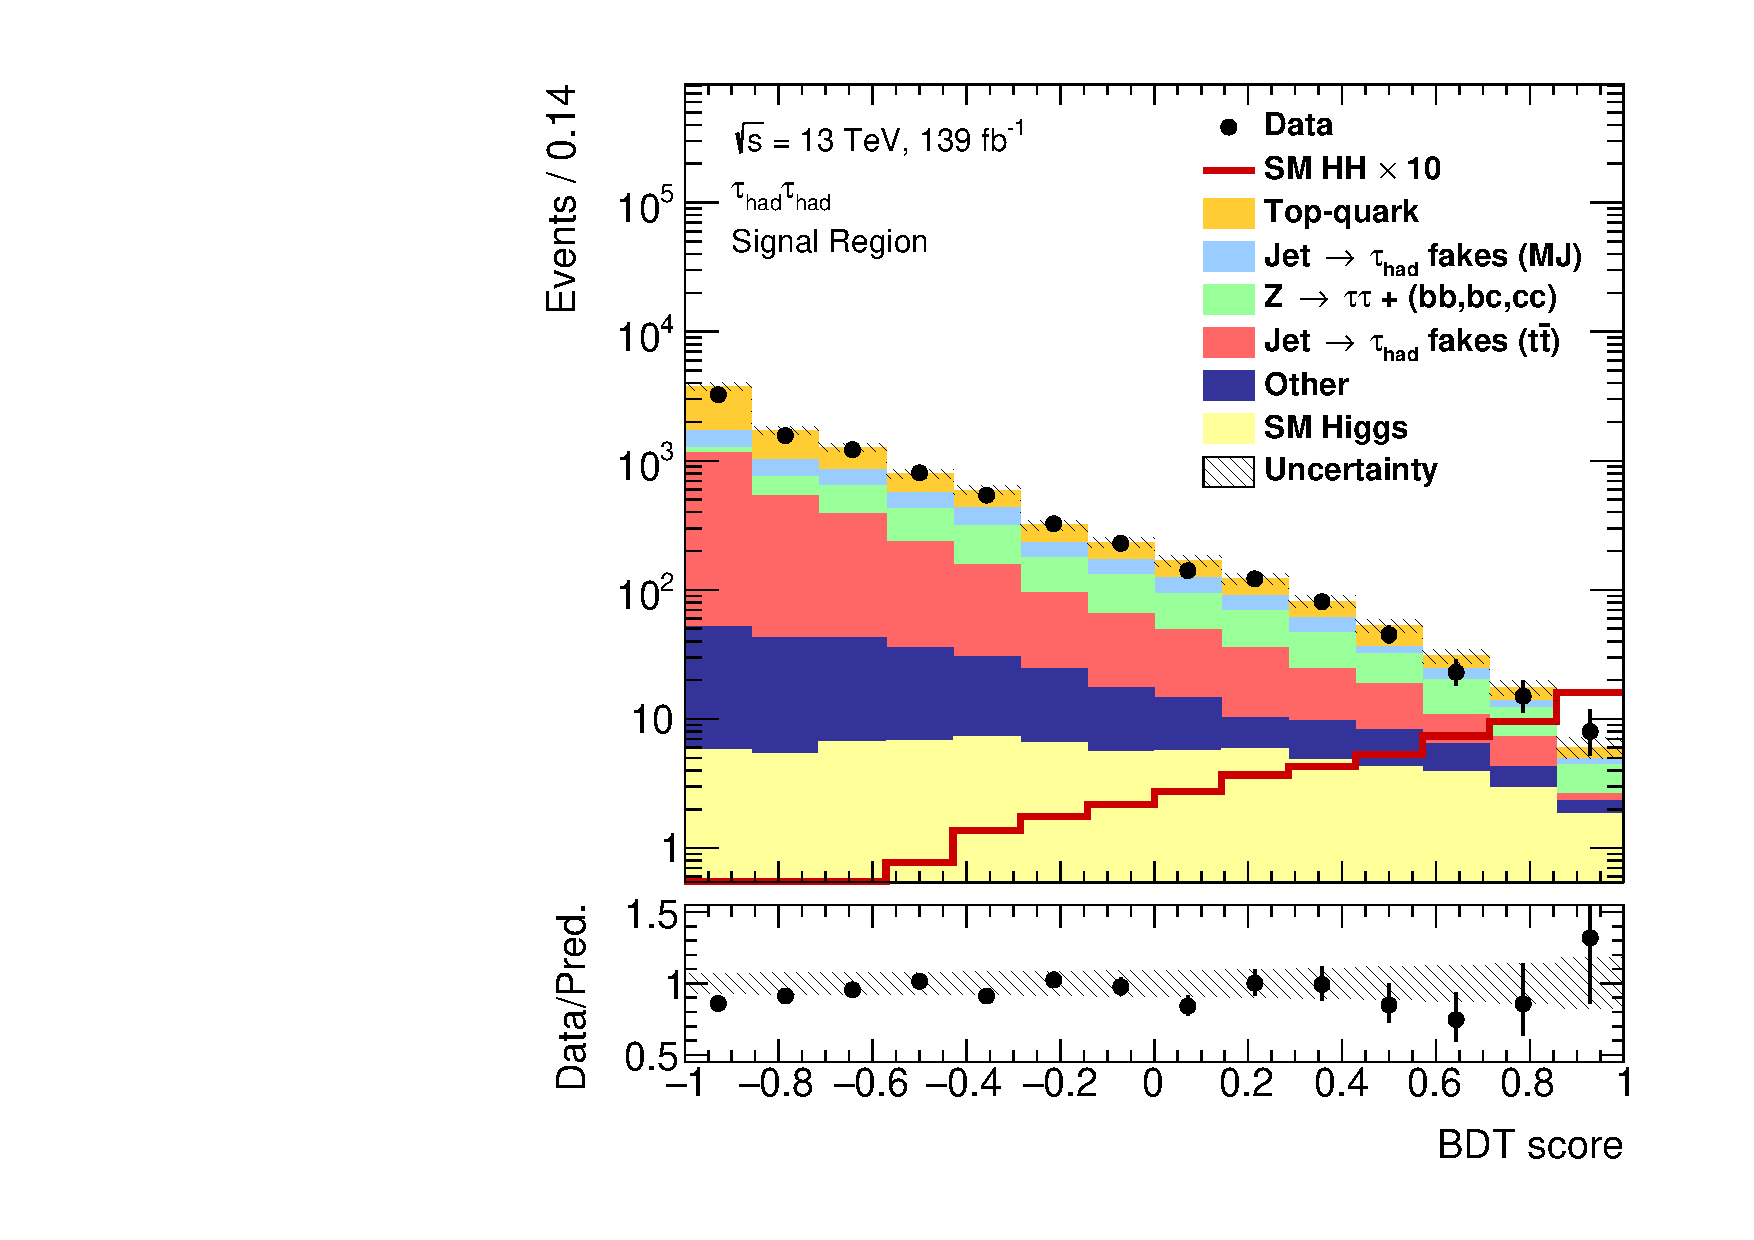
\includegraphics[width=0.6\textwidth]{mva/prefit/Region_BMin0_incJet1_distSMBDT_J2_Y2015_DLLOS_T2_SpcTauHH_L0_Prefitlog}

  \caption{Distribution of the BDT score used to select the SM \HH
    signal in the SR of the \hadhad channel prior to the maximum
    likelihood fit. The uncertainty bands include all statistical and
    systematic uncertainties of the background model. The
    normalisation of the SM \HH signal is scaled by 10 for
    illustration purposes. The choice of binning for the histograms
    will be discussed in~\Cref{sec:binning_alg}.}
  \label{fig:mva_smbdt_prefit}
\end{figure}

The sensitivity to the SM \HH signal is driven by the last bins of the
BDT score histogram.  The expected number of signal (background)
events in the two most signal-like bins is 2.6 (24) out of 5.6 (9200)
events entering the pre-selection region. With respect to the to the
pre-selection region, this selection provides a background rejection
of two orders of magnitude, $1 / \varepsilon_{\text{b}} \approx 380$,
while selecting almost half of the signal events.

The single largest background in the last two BDT score bins, with an
expectation of 6.9 events, is associated production of
$\PZ \rightarrow \tautau$ with jets originating from heavy-flavour
quarks.

The production of single Higgs bosons represents the second most
abundant background in the signal-like bins of the final
discriminant. The primary source being~$\PHiggs \rightarrow \tautau$
with about equal contribution from the gluon fusion, $\PZ\PHiggs$, and
$\ttbar\PHiggs$ production modes. A small fraction of
\SI{15}{\percent} is originating from $\PHiggs \rightarrow \bbbar$ in
associated production with a \PZ boson. The kinematic properties of
single Higgs boson production, particularly in the $Z\PHiggs$ mode, is
similar to the non-resonant \HH signal and largely limited by the
\PHiggs-system mass reconstruction performance such that about 1 in 15
single Higgs boson events in the pre-selection region are selected
into one of the two most signal-like bins, with an expectation of 4.8
events.

Other backgrounds populating the two most signal-like bins in BDT
score are originating from \ttbar (true \tauhadvis) with an
expectation of 4.6 events and \jettotauhadvis from multi-jet and
\ttbar production with 2.2 and 3.4 expected events, respectively. The
signal and background yields including all experimental and
theoretical uncertainties will be summarised
in~\Cref{sec:statistical_analysis}.

The importance of input variables in the BDT can be estimated using
the \emph{permutation importance} technique. It is a method to inspect
the importance of input variables for predictions of a black box
estimator, derived from a importance measure introduced
in~\cite{breiman01} for random forests. To inspect the importance of a
feature in a given model, the feature's values are permuted over all
instances and classes, breaking the relationship between the feature,
class labels, and other correlated input variables. The importance of
a given feature can be estimated by measuring the degradation in the
quality of the model's predictions after permuting the feature.

This technique measures the importance of a variable in a given model,
which not necessarily corresponds to the importance of the variable in
solving the underlying predictive problem. In the presence of highly
collinear features this means that some importance can be assigned to
multiple related variables even if a strict subset of variables
contains the information relevant to the problem. This effect needs to
be considered when interpreting rankings based on the permutation
importance.

In~\Cref{tab:variable_importance_bdt} a ranking of the input variables
to the BDT for the SM \HH signal is shown based the change in ROC-AUC
according to the permutation importance approach. The \PHiggs-system
masses are the most important inputs to the BDT, contributing with
approximately equal importance due to similar mass reconstruction
performance of \mMMC and \mBB. In the non-resonant production mode,
the \HH-system mass is of lesser importance due to the similarities of
the \mHH spectra between signal and background
(cf.~\Cref{fig:mva_inputs}).

\begin{table}[htbp]
  \centering

  % ["mBB", "mMMC", "mHH", "dRBB", "dRTauTau"]
% array([-0.08482375, -0.08992436, -0.03412635, -0.01212749, -0.03253109])
% (Pdb) p deltaROCAUC.mean(axis=1)
% array([-0.08560703, -0.09098586, -0.03392883, -0.01171693, -0.03247466])
% (Pdb) p deltaROCAUC.std(axis=1, ddof=1)
% array([0.00083227, 0.00054534, 0.00032627, 0.00020416, 0.00068158])

\begin{tabular}{lS}
  \toprule
  Variable & $\Delta\text{ROC-AUC}$ \\
  \midrule
  \mMMC & -0.090 \\
  \mBB & -0.085 \\
  \mHH & -0.034 \\
  \dRtautau & -0.033 \\
  \dRbb & -0.012 \\
  \bottomrule
\end{tabular}

%%% Local Variables:
%%% mode: latex
%%% TeX-master: "../../phd_thesis"
%%% End:


  \caption{Importance of the input variables in the BDT measured as
    the change in ROC-AUC when permuting the values of a single
    variable over all events. The mean $\Delta\text{ROC-AUC}$ over 10
    permutations is displayed. The statistical uncertainty is below
    0.001 and therefore omitted.}
  \label{tab:variable_importance_bdt}
\end{table}


\subsection{Extraction of resonant \HH production with Parametric
  Neural Networks}
\label{sec:mva_pnn}

The search for \HH production via scalar resonances considers
resonance masses ranging from \SI{251}{\GeV} up to \SI{1600}{\GeV},
probing a wide range of kinematic configurations of the final state
particles. As a result, the joint probability density of the
discriminating variables for signal varies with the resonance
mass. This is particularly prominent in the marginal distributions of
\mHH, \dRtautau, and \dRbb, previously shown in~\Cref{fig:mva_inputs}
for three \mX hypotheses, where the overlap between the signal and
background spectra changes as \mX is varied. This dependency needs to
be exploited to achieve optimal sensitivity when selecting signal-like
events for different signal hypotheses.

Using multivariate classifiers for signal extraction, one possible
method of incorporating the \mX dependency of the classification
problem is to train a classifier for every signal hypothesis. In this
approach multiple classification tasks are solved in isolation,
ignoring the more general classification problem. This was previously
explored in~\cite{HIGG-2016-16-witherratum} using BDT.

An alternative approach is provided by parametrised classifiers where
the dependency of the prediction problem is incorporated during
training, thus aiming to solving it in the broader context. In
particular Parametric Neural Networks (PNN)~\cite{Baldi:2016fzo} are
used due to the ability of neural networks to smoothly approximate
large classes of continuous functions. Due to these properties it is
shown in~\cite{Baldi:2016fzo} that PNN are able to interpolate the
classification task to parameter values not seen in training.

In this search PNN are implemented as feedforward neural networks
where, in addition to the five discriminating variables, the parameter
value specifying the classification task is provided as an input to
the network. During training, the value of the parameter is assigned
to be the generator-level \mX for signal events and random,
uninformative values for background events. Otherwise, PNN are
amenable to the methods commonly employed to train non-parametrised
feedforward neural networks. At evaluation time the parameter value is
held fixed according to the classification problem that should be
solved.


\subsubsection{Implementation and hyperparameter optimisation}

The PNN is trained using simulated signal events of 19 different mass
hypotheses of the scalar resonance (cf.~\Cref{tab:monte_carlo}). An
additional point at $\mX = \SI{375}{\GeV}$ was included at a later
stage of the analysis and was not part of the training and
optimisation process. The same treatment of background processes as
described in the previous section is used. The non-resonant production
of \HH predicted by the SM is not included as a background.
% Because it has not yet been observed
The signal samples are combined, ensuring that every \mX hypothesis
contributes with the same total event weight to the combined sample,
subsequently normalising the combined signal and background sample to
have equal weight. The 5-fold CV approach\todo{Mention it is
  stratified?} is used for model selection.

The training proceeds by minimising the binary cross-entropy loss
using stochastic gradient descent with momentum and exponential
learning rate decay. As part of the training process the
discriminating variables are centered and scaled by subtracting the
median and dividing by the interquartile range of the variable for
better conditioning of the loss minimisation. Similarly, the values of
the mass parameter are transformed into $[0, 1]$. The values of the
mass parameter for background events is sampled from the distribution
of \mX in the combined signal sample and is re-sampled after every
training epoch.

The neural networks consist of multiple fully-connected layers with
ReLU activation, except for the final layer which uses sigmoid
activation. The training is implemented in \textsc{Keras}~\cite{keras}
using the \textsc{TensorFlow}~\cite{tensorflow2015-whitepaper}
backend. Trained PNN are evaluated using \textsc{lwtnn}~\cite{lwtnn}.

The PNN hyperparameters are optimised using the random grid search
with nested cross validation approach used for the BDT targeting
non-resonant \HH production. The parameter grid is defined
in~\Cref{tab:hyperparameter_grid_pnn}. To reduce the dimensionality of
the hyperparameter space, the number of neurons in the hidden layers
except for the first and last hidden layers are required to be the
same.

\begin{table}[htbp]
  \centering
  \begin{tabular}{ll}
  \toprule
  Hyperparameter & Values considered \\
  \midrule
  Epochs & 50, 100, \underline{200}, 400 \\[0.1em]
  Batch size & 64, \underline{128}, 256 \\[0.1em]
  Learning rate & 0.01, 0.02, 0.05, 0.1, \underline{0.2} \\[0.1em]
  Learning rate decay & $10^{-6}$, \underline{$10^{-5}$}, $10^{-4}$, $10^{-3}$ \\[0.1em]
  Number of hidden layers & 1, 2, 3, \underline{4}, 5 \\[0.1em]
  Layer size (first hidden layer) & 16, 32, 64, \underline{128} \\[0.1em]
  Layer size (last hidden layer$^*$) & \underline{16}, 32, 64, 128 \\
  Layer size (other hidden layers$^\dagger$) & 16, 32, 64, \underline{128} \\[0.1em]
  \bottomrule
\end{tabular}

%%% Local Variables:
%%% mode: latex
%%% TeX-master: "../phd_thesis"
%%% End:

  \caption{Parameter values used to defined the grid of
    hyperparameters considered for the optimisation of the PNN
    configuration. Parameters marked with $*$ and $\dagger$ are only
    applicable when the number of hidden layers is larger than 1 and
    2, respectively. The underlined values show the final PNN
    configuration after hyperparameter optimisation.}
  \label{tab:hyperparameter_grid_pnn}
\end{table}

No clear choice of optimisation metric exists to evaluate a continuum
of related classification task. For simplicity, the ROC-AUC of the PNN
when performing binary classification of a resonant signal with
$\mX = \SI{325}{\GeV}$ against background is chosen. This choice is
motivated by the strength of the $\PX \to \HH \to \bbtautau$ search
channel in an intermediate mass range of the scalar resonance from
approximately \SI{300}{\GeV} to \SI{600}{\GeV} compared to other
channels in $\bbbar\gamma\gamma$ and $\bbbar\bbbar$ final states which
are expected dominate the low and high \mX signal sensitivity,
respectively. The similarity of the \HH signal from resonant
production with the bulk of the background is largest at low resonance
masses, thus a lower value of \mX in the considered range is selected.

About 1600 unique configurations of the PNN are tested, the 400
highest ranking in ROC-AUC showing compatible performance in terms of
the performance estimate obtained from CV. A single configuration is
obtained by choosing the best performing parameter set in CV on
even-numbered events and using the same configuration for odd-numbered
events. The chosen configuration, underlined
in~\Cref{tab:hyperparameter_grid_pnn}, has a ROC-AUC in 5-fold CV of
\num{0.9764 +- 0.0009} on even- and \num{0.9754 +- 0.0009} on
odd-numbered events\footnote{On the dataset with odd-numbered events
  the chosen configuration is the 54th highest ranking one in terms of
  the ROC-AUC. For comparison, the highest ranking model on
  odd-numbered event has a ROC-AUC of \num{0.9761 +- 0.0020}, showing
  compatible performance with the chosen configuration.}. The PNN are
then re-fit on all five folds of the inner CV separately for even- and
odd-numbered events.

\subsubsection{Evaluation of PNN performance}

In~\Cref{fig:pnn_score_prefit} the PNN score is shown evaluated in the
\hadhad signal region with a \mX parameter of 300, 500 and
\SI{1000}{\GeV} on the withheld data. The PNN is able to select the
signal of interest given the parameter is set to the corresponding
value. Depending on the classification task the PNN is solving,
diffent backgrounds populate the most signal-like region at high MVA
score.

\begin{figure}[htbp]
  \centering

  \begin{subfigure}[t]{.49\textwidth}
    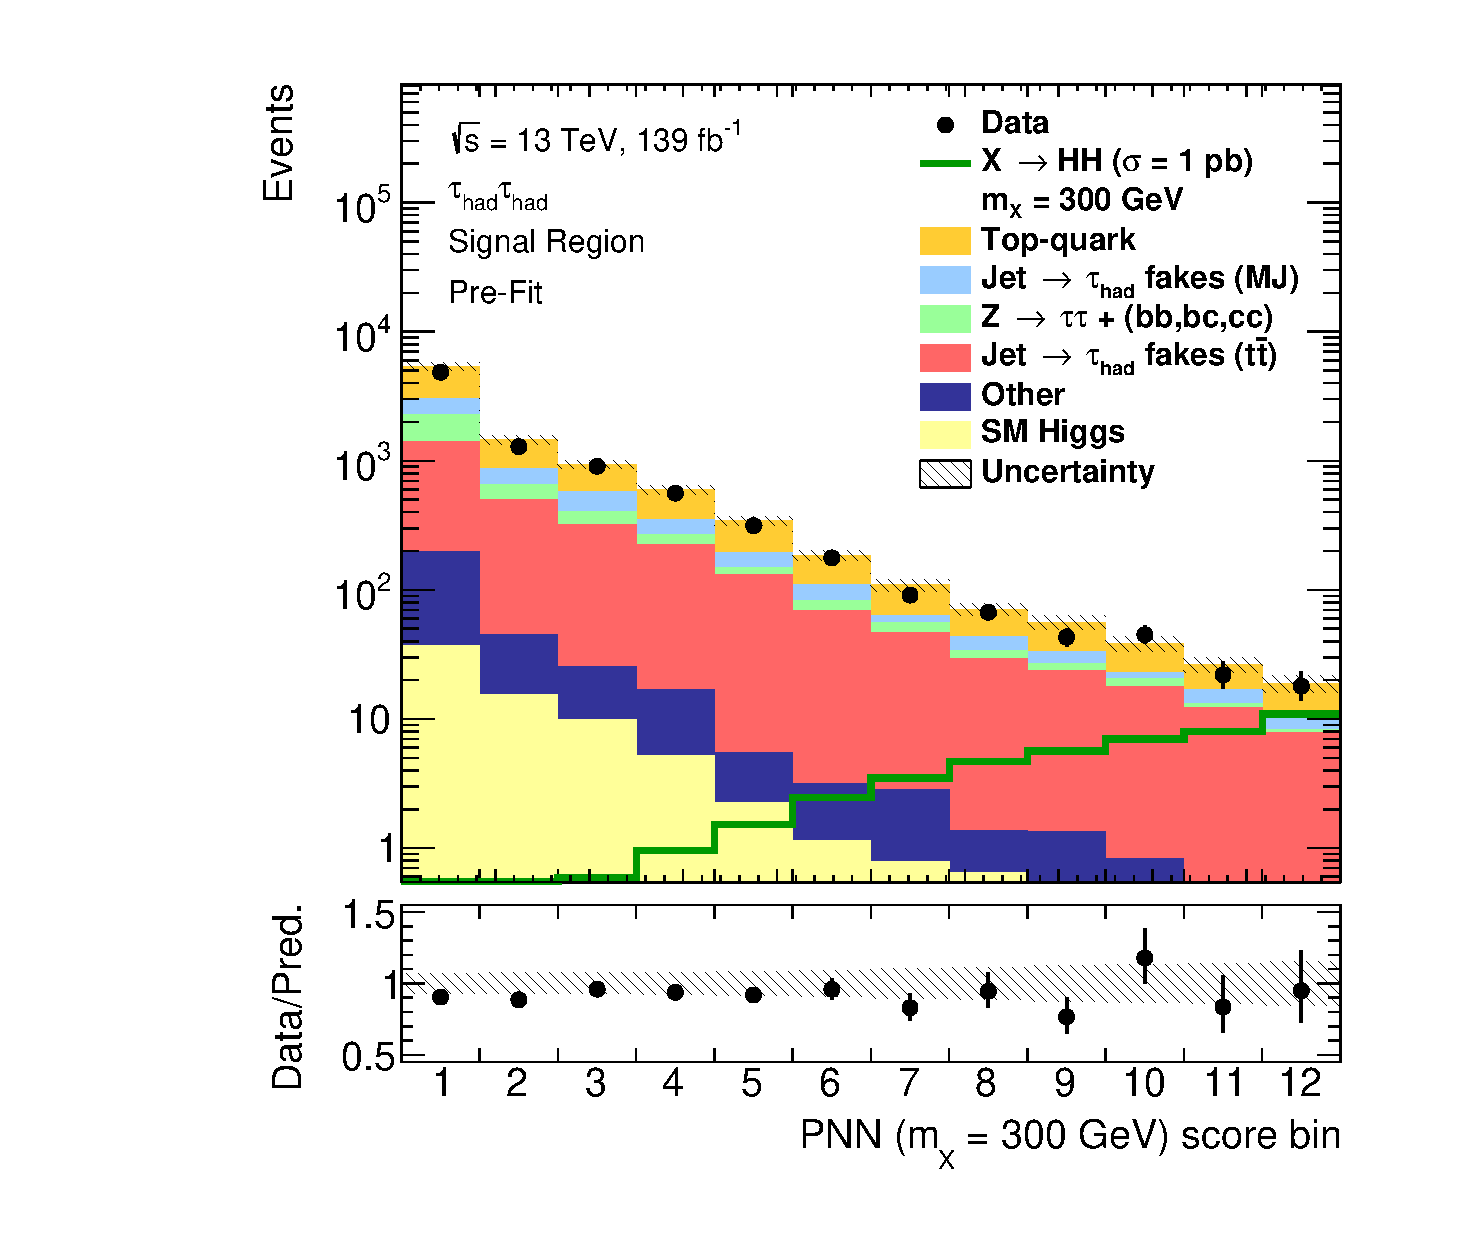
\includegraphics[width=\textwidth]{mva/prefit/Region_BMin0_incJet1_distPNN300_J2_Y2015_DLLOS_T2_SpcTauHH_L0_Prefit_logy}
    \caption{}
    \label{fig:pnn_score_prefit_300}
  \end{subfigure}\hfill%
  \begin{subfigure}[t]{.49\textwidth}
    \centering
    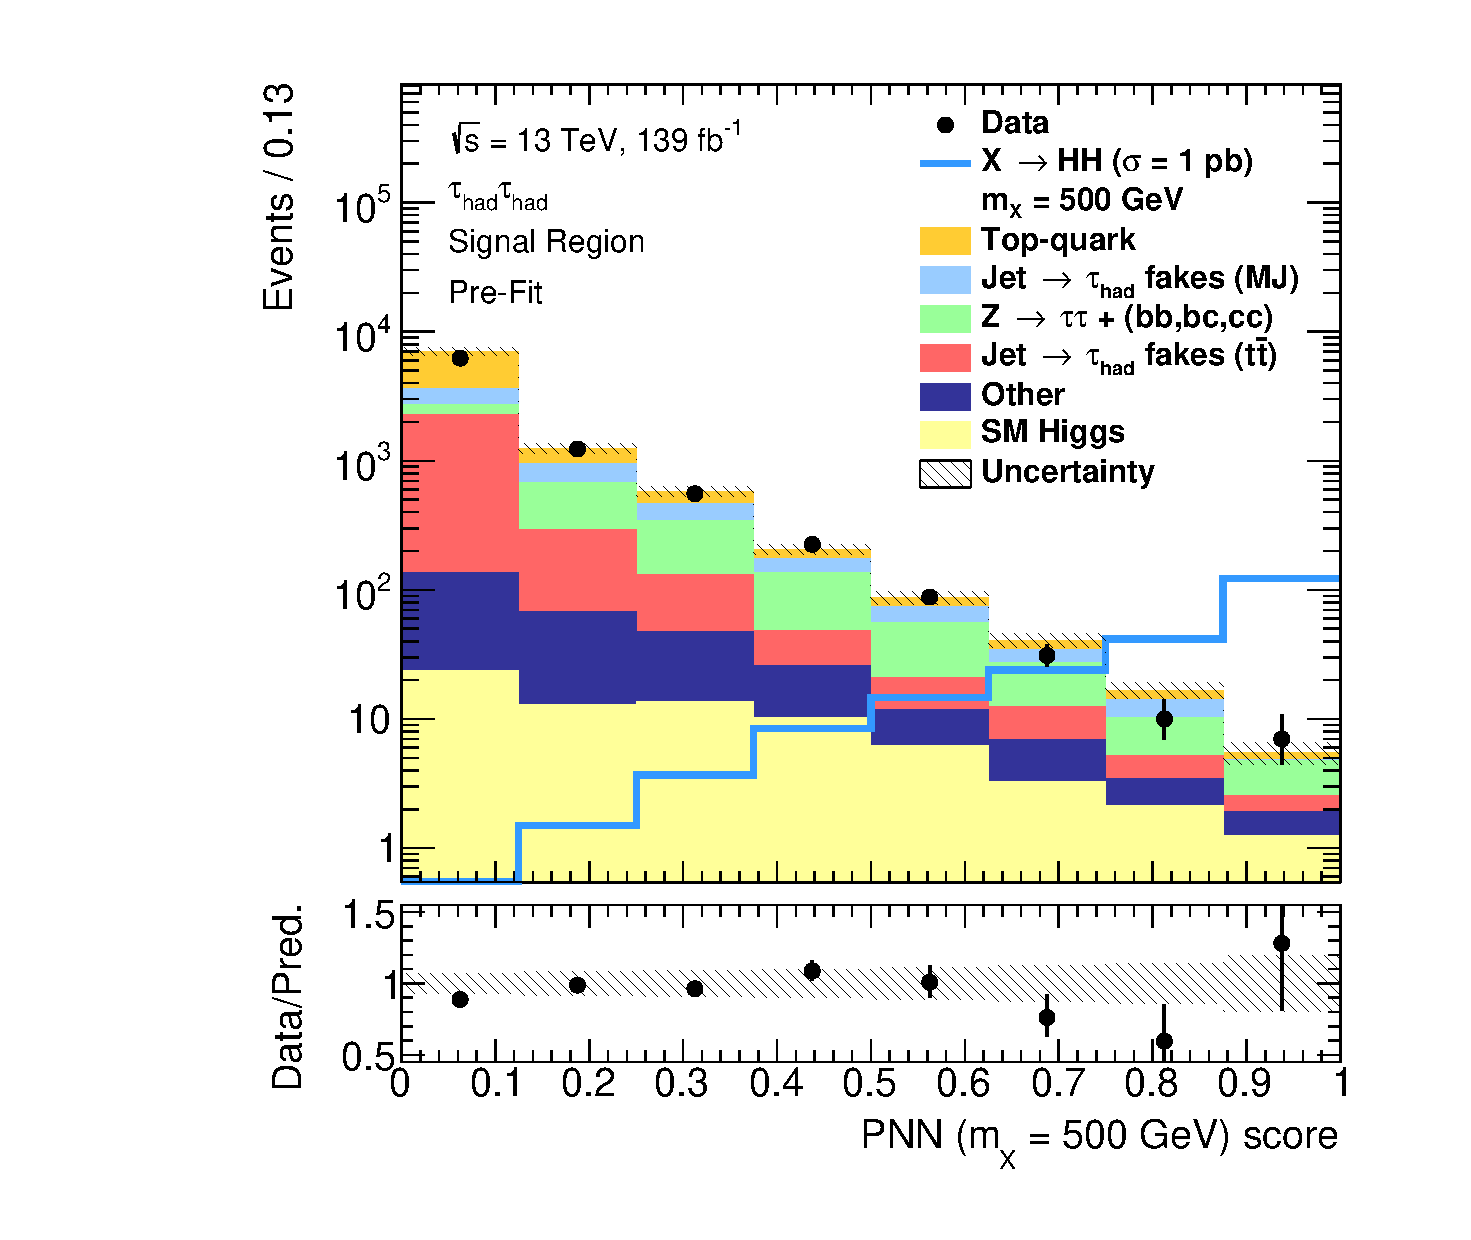
\includegraphics[width=\textwidth]{mva/prefit/Region_BMin0_incJet1_distPNN500_J2_Y2015_DLLOS_T2_SpcTauHH_L0_Prefit_logy}
    \caption{}
    \label{fig:pnn_score_prefit_500}
  \end{subfigure}

  \begin{subfigure}[t]{.49\textwidth}
    \centering
    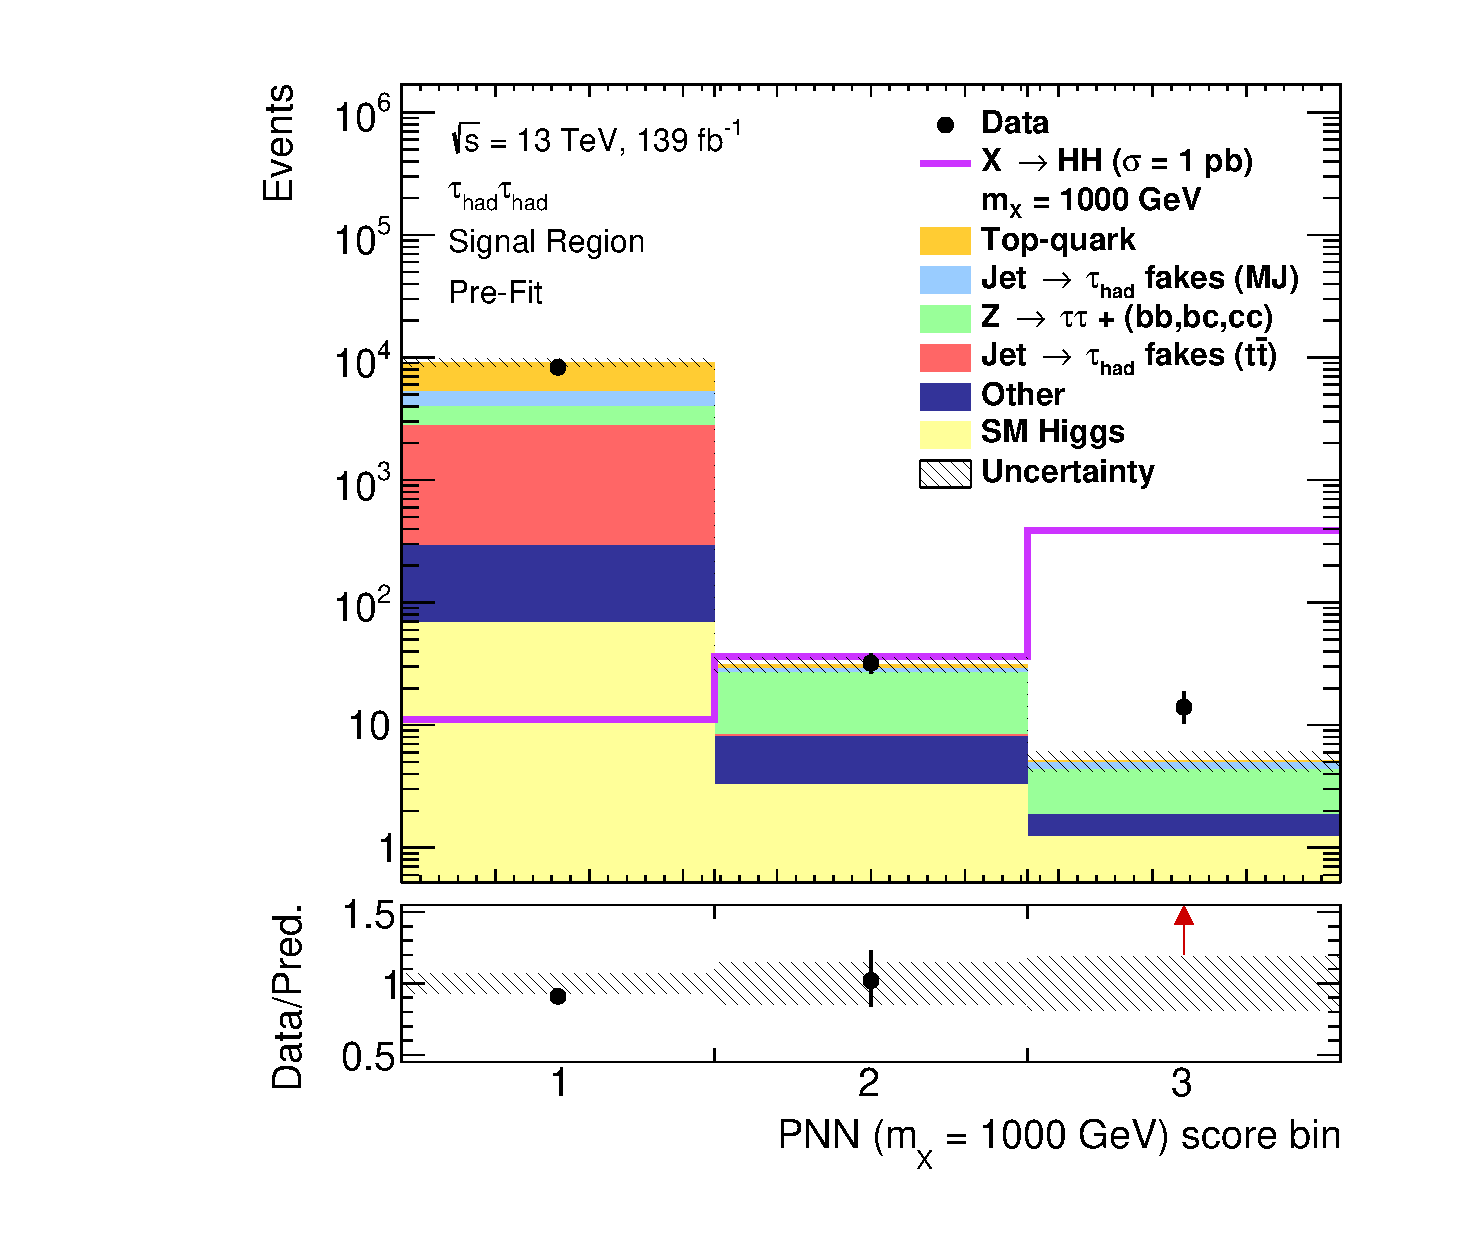
\includegraphics[width=\textwidth]{mva/prefit/Region_BMin0_incJet1_distPNN1000_J2_Y2015_DLLOS_T2_SpcTauHH_L0_Prefit_logy}
    \caption{}
    \label{fig:pnn_score_prefit_1000}
  \end{subfigure}

  \caption{Distribution of the PNN score evaluated with PNN mass
    parameters set to \SI{300}{\GeV} (a), \SI{500}{\GeV} (b), and
    \SI{1000}{\GeV} (c) prior to the maximum likelihood fit.  The
    signal overlay is normalised to a cross-section of
    $\Pproton\Pproton \to \PX \to \HH$ of \SI{1}{\pico\barn}. The
    choice of binning and excess in data for he the most signal-like
    bin of the PNN ($\mX = \SI{1000}{\GeV}$) score will be discussed
    in a later sections (REFERENCE).}
  \label{fig:pnn_score_prefit}
\end{figure}

When searching for resonances of low mass, for example \SI{300}{\GeV}
shown in~\Cref{fig:pnn_score_prefit_300}, the dominant background in
the two most signal-like bins is \ttbar with both true and
\faketauhadvis with \SI{80}{\percent} of the total background. At
intermediate masses of around \SI{500}{\GeV} the background
contribution is similar to the non-resonant \HH case in the SM due to
it having an average \mHH of about \SI{500}{\GeV} after pre-selection.
At high masses, the signal-like bins are populated predominately by
boosted $\PZ \to \tautau$ recoiling against jets of heavy flavour.

The two previously highlighted properties of the PNN, the ability to
solve a continuously varying classification parametrised by \mX and
the ability to interpolate to values of \mX not seen during training,
are investigated in the following. For this investigation an
approximation of the expected signal significance is used. The PNN
score distribution for a given setting of the parameter and a given
benchmark signal is binned according to an automatic binning algorithm
that will be formally introduced in~\Cref{sec:binning_alg} that aims
to yield high signal sensitivity while limiting the impact of
background statistical uncertainties and ensuring reasonable validity
of asymptotic approximations. The approximate significance of a
Poisson counting experiment in the absence of uncertainties on the
signal and background expectations,
$\nu_\text{s} / \sqrt{\nu_\text{b}}$, of all bins is added in
quadrature. This sum will be dominated by the most signal-like bins of
the PNN score distributions.

This metric is used in~\Cref{fig:pnn_detuning} by inspecting the
significance of a given benchmark signal as the mass parameter of the
PNN is varied. The highest expected significance for a given benchmark
results when the PNN's parameter is set to the resonance mass of the
benchmark signal. The width of the significance curves also reflect
the mass sensitivity of the MVA analysis strategy. Note that this
method is aimed at the discovery of a signal and thus does not perform
optimally in terms of the mass resolution. This can be seen in FIGURE,
where the width of XXX is shown which is much larger than the
intrinsic resolution on mHH at high mass. In case of a discovery a new
analysis would be needed to more accurately predict the resonance
mass.

The interpolation property is checked, \Cref{fig:pnn_interpolation},
by removing signals from the training and comparing the significance
response for a given signal that was excluded in training. Testing the
removed significances yielded close to the same peak significance as
in the training that included the point.  This motivates the use of
the PNN also for the 375 GeV mass point which was added to fill a gap
in mass sensitivity (seen in~\Cref{fig:pnn_detuning}) where it could
be possible to miss a signal.

\begin{figure}[htbp]
  \centering

  \begin{subfigure}[t]{.49\textwidth}
    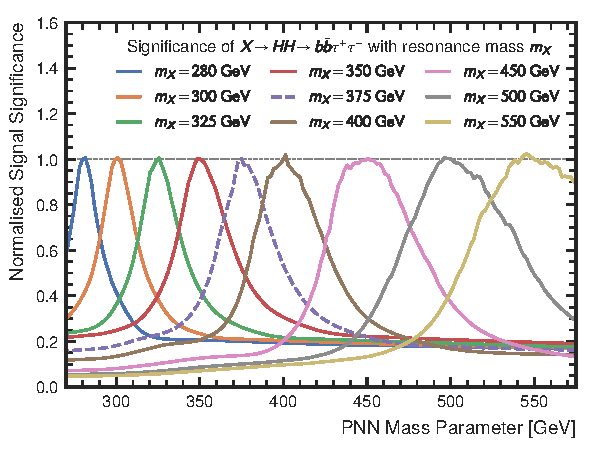
\includegraphics[width=\textwidth]{mva/detuning}
    \caption{Response of final PNN configuration used in the search
      for resonant production of \HH.}
    \label{fig:pnn_detuning}
  \end{subfigure}\hfill%
  \begin{subfigure}[t]{.49\textwidth}
    \centering
    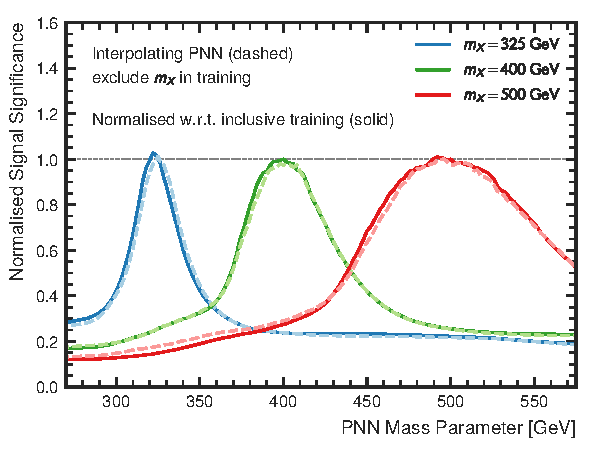
\includegraphics[width=\textwidth]{mva/interpolation}
    \caption{Comparison of PNN before hyperparameter optimisation when
      including (solid) and excluding (dashed) certain resonance
      masses in training.}
    \label{fig:pnn_interpolation}
  \end{subfigure}

  \caption{Expected signal significance of a scalar resonance with
    mass \mX as a function of the PNN mass parameter. The significance
    is estimated by binning the PNN score for a given value of the
    parameter and adding the Asimov significance of all bins in
    quadrature. Only statistical uncertainties are considered. The
    binning is determined by an algorithm that will be described
    in~\Cref{sec:binning_alg}. The curves are scaled such that the
    significance is 1 when the PNN mass parameter is equal to \mX of
    the hypothesis under test. Dashed lines correspond to signal mass
    hypotheses that were not included in the PNN training.}
  \label{fig:pnn_properties}
\end{figure}


%%% Local Variables:
%%% mode: latex
%%% TeX-master: "../../phd_thesis"
%%% End:
